\chapter{Levantamento Bibliográfico} \label{cap:funda}

Nessa seção será descrito o estado da arte do tema escolhido. Primeiramente será dado uma breve história do desenvolvimento dos quadricópteros e, em seguida, serão apresentados os trabalhos correlatos recentes.

\section{História dos quadricópteros}

O desenvolvimento dos primeiros quadricópteros começou a mais de um século. Em 1907, os irmãos franceses Louis e Jaques Breguet construíram o primeiro quadricóptero pilotado, chamado de \textit{Gyroplane nº 1} \cite{leishman00}. A estrutura era constituída por quatro vigas, formadas de tubos de aço, dispostas em formato de cruz e com um lugar para o piloto ao centro, próximo ao motor. No entanto, devido a falta de estabilidade e de meios de controle, ele só foi capaz de levantar voo por alguns segundos.

Nas décadas seguintes houve grandes avanços em desempenho e controle dos quadricópteros. Em 1922, G. de Bothezat, um imigrante russo nos Estados Unidos, conseguiu realizar vários voos a baixas altitudes e baixas velocidades. Em 1924, o francês E. Oehmichen recebeu um prêmio da \sigla{FAI}{Federação Aeronáutica Internacional} por demonstrar um voo do seu quadricóptero em um circuito fechado de 1 km, com duração de 7 minutos e 40 segundos. Foi o primeiro helicóptero conseguir percorrer essa distância. Ambos os projetos foram cancelados por serem impraticáveis para uso real e pelo alto custo de desenvolvimento.

Alguns anos depois, em 1956, nos Estados Unidos, o Convertawings Modelo A reviveu os projetos de Bothezat e Oehmichen \cite{lambermont58}. Inventado por D. H. Kaplan, esse quadricóptero tinha os quatro rotores posicionados em forma de ``H'', ao invés de ``+'', como nos anteriores. Apesar de ter sido testado com sucesso, o apoio do Exército dos EUA foi encerrado.

O interesse pelos quadricopteros caiu com o início da comercialização de helicópteros convencionais, de um ou dois rotores, e só foi retomado na década de 90, desta vez no contexto de VANTs.

\subsection{Teste de Terceiro Nível}

%
aaaa

\begin{figure}[htb]
	\centering
	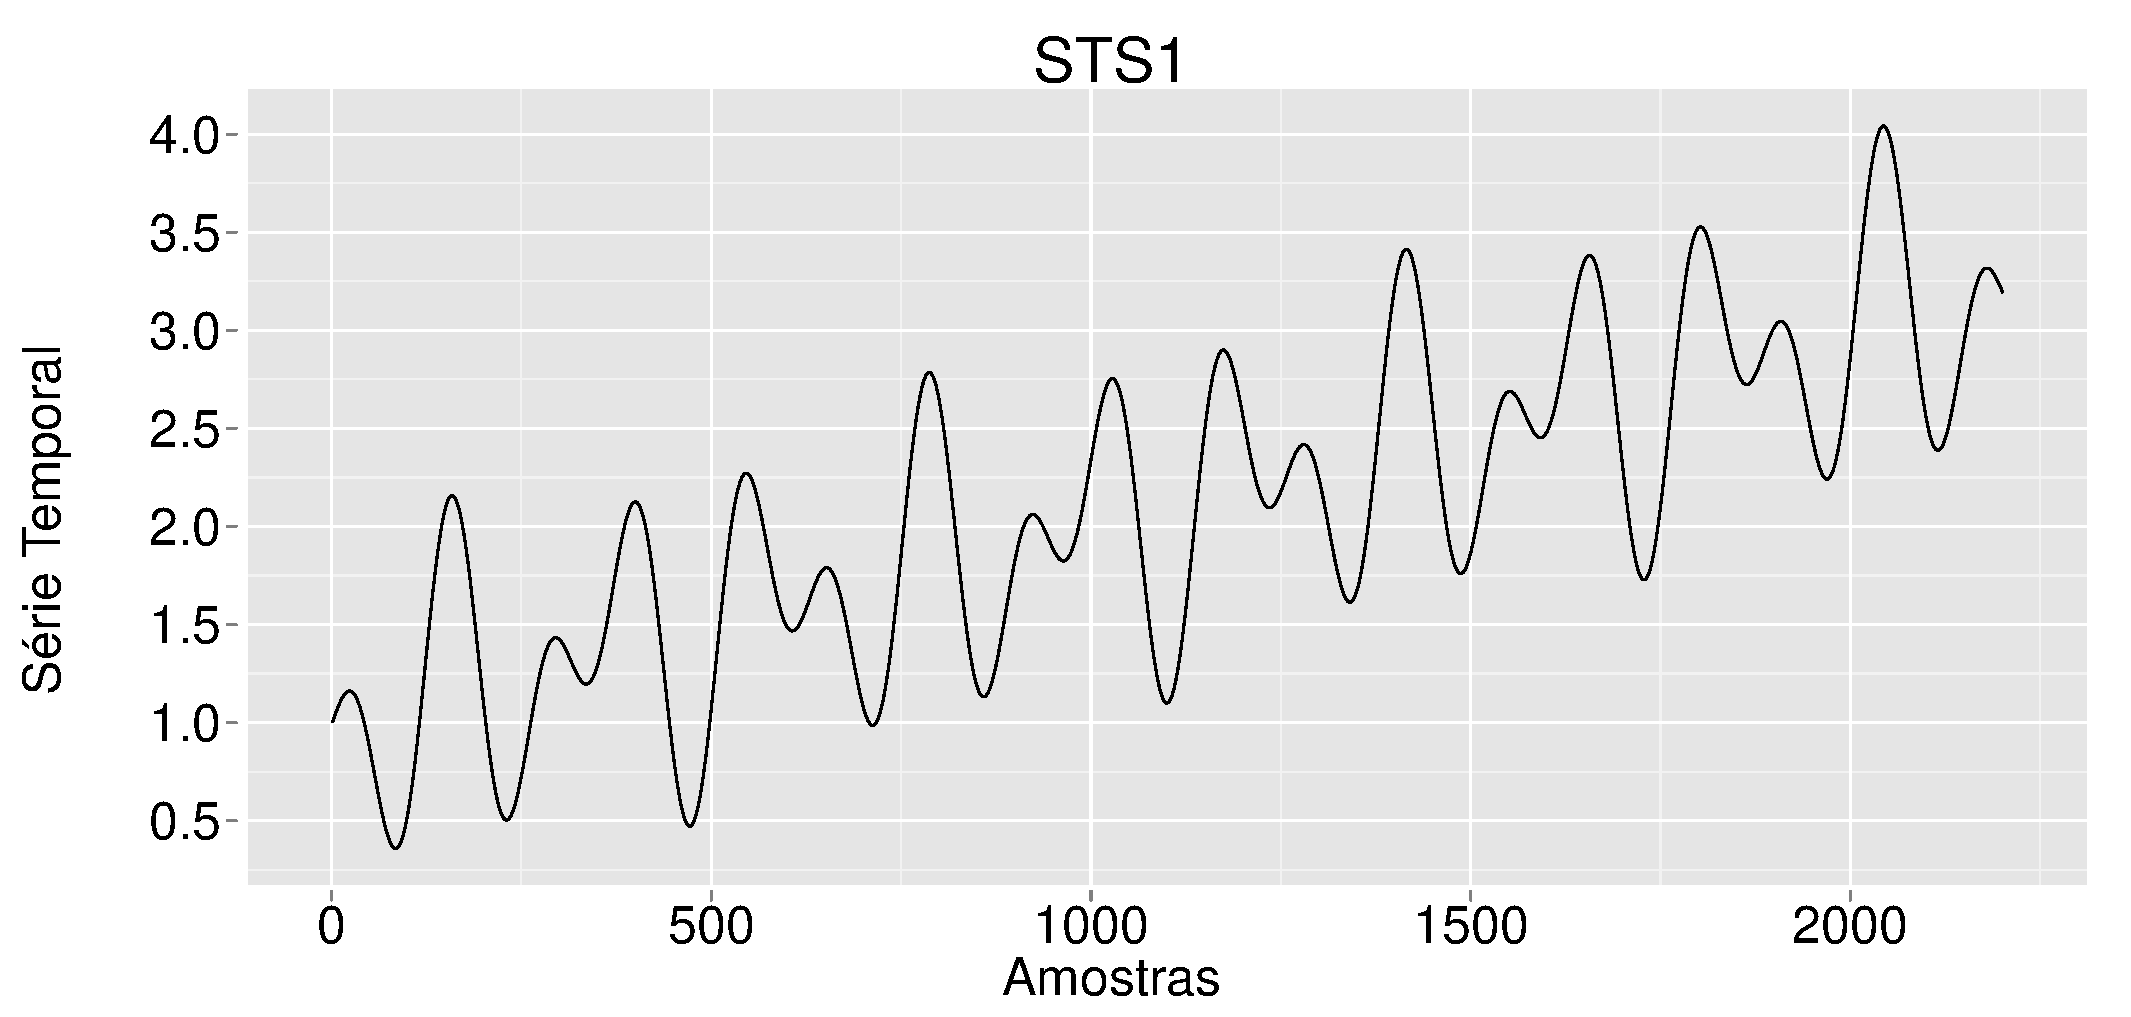
\includegraphics[width=0.4\textwidth]{Imagens/Arta1} % <- formatos PNG, JPG e PDF
	\caption[Texto que vai aparecer na lista de fig.]{Texto que vai aparecer embaixo da imagem.}
\fonte{\citeonline{AikesJunior2011}}%citaç\~ao do livro onde pegou a figura	
	\label{fig:tux_laplace}
\end{figure}

\section{Trabalhos correlatos}

Os desenvolvimentos recentes em materiais mais leves, componentes eletrônicos, motores elétricos, baterias e, principalmente, MEMS, permitiram que os VANTs se tornassem realidade. Com isso, muitos projetos de quadricópteros foram desenvolvidos independentemente 

Um dos primeiros projetos de quadricóptero VANT publicados foi o Hoverbot, em 1993 na Universidade de Michigan, construído basicamente pela união de quatro helicópteros de brinquedo pela cauda. O projeto foi rapidamente abandonado pelas dificuldades na construção do \textit{hardware}, mas conseguiu planar com o auxílio de uma estrutura que inibia seus movimentos horizontais \cite{borestein93}.

O projeto Mesicopter, desenvolvido em 2001 na Universidade de Stanford, buscava desenvolver quadricópteros na escala de centímetros e com massa de 3 a 15g. Sua aplicação seria para coleta de dados atmosféricos ou metereológicos em grandes áreas ou planetas. No entanto, ele nunca foi capaz de levantar o peso da sua fonte de alimentação \cite{kroo01}.

Em 2002, na Universidade da Pensilvânia, E. Altug desenvolveu um quadricóptero baseado em realimentação visual. O sistema de visão usa câmeras no solo para estimar a posição e a orientação, baseado em círculos coloridos dispostos no veículo, que servem de entrada para o sistema de controle, cuja saída é enviada ao quadricóptero. Duas técnicas de controle foram testadas: \textit{feedback linearization} e \textit{backstepping}. O veículo utilizado foi baseado no brinquedo HMX-4 \cite{altug02}.

Outro estudo foi a dissertação de mestrado de E. B. Nice, realizado em 2004 na Universidade de Cornell. Seu trabalho envolveu desenvolvimento completo da estrutura e controle. Foram utilizados um Filtro Sigma Point para estimar o estado e um controle LQR para estabilização. O veículo final pesava 6,2 kg. Durante os testes foi comprovada sua capacidade de planar a uma altura fixa, porém não foi possível completar os testes devido a falhas no \textit{hardware} \cite{niceCU04}. O projeto teve continuidade com o trabalho de Oliver Purwin, em 2009, no qual foi utilizado \textit{Iterative Learning Control} (\sigla{ILC}{Iterative Learning Control}, do inglês, controle por aprendizado iterativo) para realizar manobras agressivas \cite{purICRA09}. Desta vez não ocorreram problemas e os testes foram bem sucedidos.

Em 2003, no Instituto Federal de Tecnologia da Suíça , S. Bouabdallah começou o desenvolvimento de um quadricóptero chamado OS4. O projeto visava um sistemático processo de modelagem, desenvolvimento e controle de helicópteros miniatura, o qual foi aplicado no OS4. Foram testados cinco tipos de controladores: baseado na teoria de Lyapunov, \sigla{PID}{Proporcional Integral Derivativo} (Proporcional Integral Derivativo), \sigla{LQ}{Linear Quadrático} (Linear Quadrático), \textit{backstepping} e \textit{sliding-mode}. Por fim, foi escolhida a técnica de \textit{backstepping} incrementada com ação integral. O projeto teve sua conclusão em 2007, com a defesa da tese de doutorado de Bouabdallah \cite{bouabdallah07}. 

Em 2004, foi criado um projeto na Universidade de Stanford com o intuito de testar e validar algoritmos de controle multi-agentes, chamado de STARMAC. Alguns campos de estudo foram: detecção de obstáculos e colisão com outros veículos, formação de voo e seguir trajetória, usando técnicas centralizadas ou descentralizadas. Para seu controle foram utilizadas três técnicas: \textit{Integral Sliding Mode}, \textit{Reinforcement Learning} e filtros de Kalman. O quadricóptero utilizado era uma modificação do brinquedo Draganflyer III, foi um dos primeiros projetos a trabalhar em ambiente externo (\textit{outdoor}). O projeto teve continuidade com em 2007, o STARMAC II, com uma versão própria do quadricóptero e com melhorias no desempenho do controlador \cite{starmac04, starmac07}.

Outros dois projetos de grande interesse, com características bem semelhantes, mas desenvolvidos independentemente, são os projetos do Laboratório GRASP da Universidade da Pensilvânia e da Flying Machine Arena do Instituto Federal de Tecnologia da Suíça. Ambos utilizam versões modificadas do quadricóptero ``Hummingbird'', vendido pela Ascending Technologies, como também o sistema de captura de movimentos Vicon, que provê a posição do quadricóptero a uma taxa de 200 Hz e com precisão milimétrica \cite{Lupashin2010, michael2010}. Ao contrário da maioria trabalhos anteriores, esses veículos não são autônomos, eles dependem de um processamento externo para calcular seu próximo movimento, reduzindo o processamento embarcado. Apesar das limitações impostas pelo sistema de câmeras, a precisão obtida permitiu a realização de tarefas complexas, inalcançáveis até hoje com os quadricópteros autônomos .

Estão em desenvolvimento novas alternativas para navegação autônoma baseadas no mapeamento em 3D do ambiente. As abordagens incluem o uso de scanners a LASER \cite{dryanovski11}, sensores Microsoft Kinect \cite{stowers11} ou ambos \cite{shen12}.

No Brasil poucos trabalhos foram publicados nesse tema. A dissertação de mestrado de \citeonline{melo2010}, da Universidade Federal do Espírito Santo, propõe um quadricóptero como plataforma para desenvolvimento de algoritmos de controle. Ele descreve os componentes utilizados, as placas microcontroladas desenvolvidas e a do software sistema embarcado implementação, fazendo a interface com o rádio, os sensores e os motores e deixando livre a implementação do algoritmo de controle. São realizados testes de comunicação, leitura dos sensores e ativação dos motores, mas nenhum algoritmo de controle é testado para validar o funcionamento completo veículo. Em \citeonline{lopes2011}, o modelo matemático de um quadricóptero é utilizado para simular e avaliar técnicas de controle. É proposto o uso de um único controlador \textit{Model Predictive Control} (\sigla{MPC}{Model Predictive Control}) para controlar posição e estabilidade do sistema, ao ínves de dois controladores separados, como visto na literatura. Os resultados são comparados com controladores PID e \textit{backstepping}, mostrando-se melhor que o primeiro e inferior ao segundo.